% 固定来源 PDF 印刷页 74 第 7 题四组选项轨迹图的矢量示意。
% 四分之一椭圆弧仅表达原图所在象限及端点，不提供额外数据。
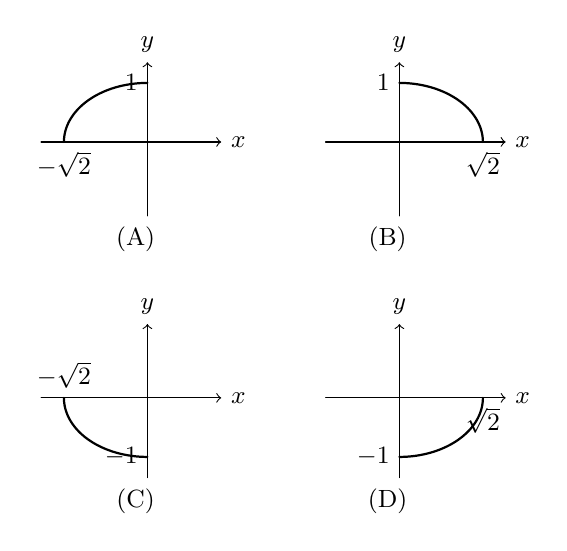
\begin{tikzpicture}[x=.75cm,y=.75cm,font=\small,line cap=round,line join=round]
  \begin{scope}
    \draw[->] (-1.8,0)--(1.25,0) node[right] {$x$};
    \draw[->] (0,-1.25)--(0,1.35) node[above] {$y$};
    \draw[thick,domain=0:90,samples=50] plot ({-1.414*cos(\x)},{sin(\x)});
    \node[below] at (-1.414,0) {$-\sqrt2$}; \node[left] at (0,1) {$1$};
    \node at (-.2,-1.65) {(A)};
  \end{scope}
  \begin{scope}[xshift=3.2cm]
    \draw[->] (-1.25,0)--(1.8,0) node[right] {$x$};
    \draw[->] (0,-1.25)--(0,1.35) node[above] {$y$};
    \draw[thick,domain=0:90,samples=50] plot ({1.414*sin(\x)},{cos(\x)});
    \node[below] at (1.414,0) {$\sqrt2$}; \node[left] at (0,1) {$1$};
    \node at (-.2,-1.65) {(B)};
  \end{scope}
  \begin{scope}[yshift=-3.25cm]
    \draw[->] (-1.8,0)--(1.25,0) node[right] {$x$};
    \draw[->] (0,-1.35)--(0,1.25) node[above] {$y$};
    \draw[thick,domain=0:90,samples=50] plot ({-1.414*cos(\x)},{-sin(\x)});
    \node[above] at (-1.414,0) {$-\sqrt2$}; \node[left] at (0,-1) {$-1$};
    \node at (-.2, -1.75) {(C)};
  \end{scope}
  \begin{scope}[xshift=3.2cm,yshift=-3.25cm]
    \draw[->] (-1.25,0)--(1.8,0) node[right] {$x$};
    \draw[->] (0,-1.35)--(0,1.25) node[above] {$y$};
    \draw[thick,domain=0:90,samples=50] plot ({1.414*sin(\x)},{-cos(\x)});
    \node[below] at (1.414,0) {$\sqrt2$}; \node[left] at (0,-1) {$-1$};
    \node at (-.2,-1.75) {(D)};
  \end{scope}
\end{tikzpicture}
